\section{Criterio di early stopping modificato}
\subsection{Introduzione}
Come step successivo si è deciso di modificare il criterio di early stopping dei modelli inserendo come variabile anche le emissioni.
Il classico criterio di early stopping prevede di fermare l'addestramento del modello quando lo score ottenuto con il validation set non migliora per un certo numero di epoche consecutive.


\begin{figure}[H]
    \centering
    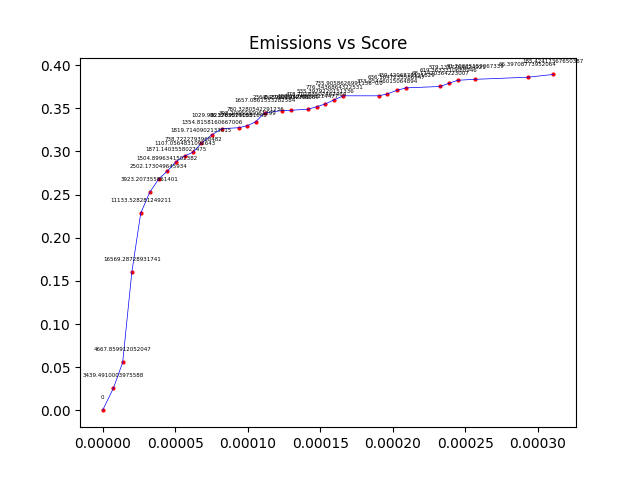
\includegraphics[scale=1]{images/curve_emissions_score.png}
    \caption{Andamento dello score in funzione delle emissioni}
\end{figure}

\noindent Questa curva mostra mostra il comportamento dello score in funzione delle emissioni. In particolare si tiene traccia solo delle epoche in cui lo score è migliorato rispetto al risultato migliore.
Si può notareee coome la curva presenti una forte crescita iniziale, per poi stabilizzarsi e avere un andamento quasi lineare.
Questo andamento lineare indica dunque un miglioramento molto piccolo dello score rispetto alle emissioni.

\noindent Il criterio di early stopping con emissioni si pone dunque come obiettivo quello di fermare l'addestramento del modello quando il miglioramento dello score rispetto alle emissioni è troppo piccolo.
L'idea alla base sarebbe quello di fermare l'addestramento studiando la derivata della curva. Siccome i valori sono discreti, si è deciso di approssimare la derivata con la differenza tra due punti consecutivi \footnote{Metodo delle differenze divise di ordine 1}{} mediante la seguente formula:
\begin{equation}
    \frac{f(x_{i+1}) - f(x_i)}{x_{i+1} - x_i}
\end{equation}

\noindent Quando la differenza tra due rapporti consecutivi è minore di una certa soglia, per un certo numero di volte consecutive, si ferma l'addestramento del modello.

\subsection{Risultati}

Il primo esperimento è stato compiuto con il dataset MovieLens-1m. La soglia è stata impostata a 50 e il numero di epoche consecutive a 5.

\begin{table}[H]
    \centering
    \footnotesize
    \setlength\tabcolsep{0pt}
    \begin{tabularx}{\textwidth}{|X|X|}
        \hline
        \textbf{Criterio classico} & \textbf{Criterio modificato} \\
        \hline
        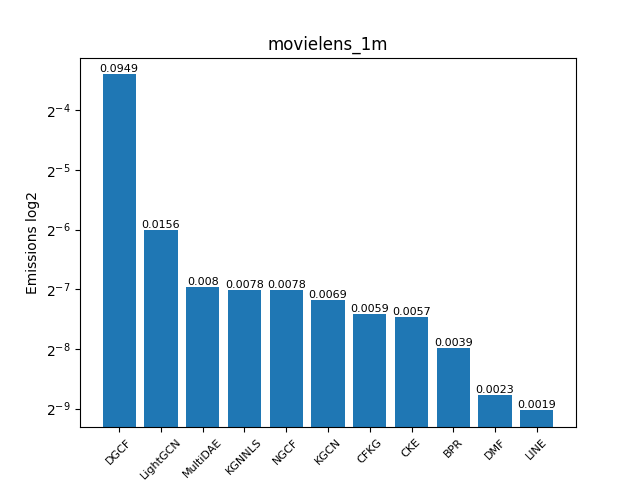
\includegraphics[width=\linewidth, trim=0 0 0 0]{images/emissions_movielens_1m_earlyClassic.png} &
        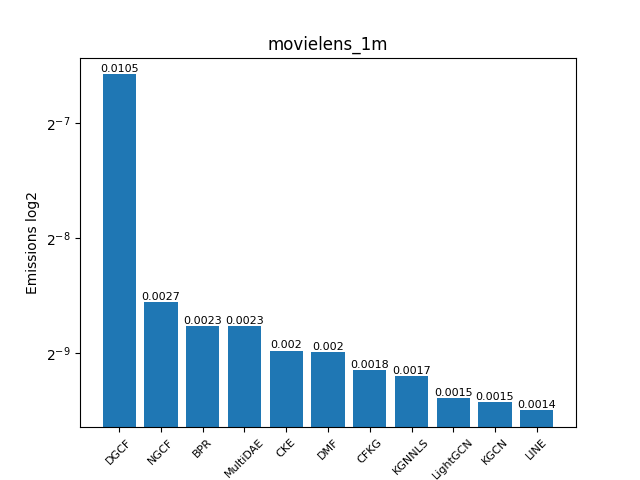
\includegraphics[width=\linewidth, trim=0 0 0 0]{images/emissions_movielens_1m_earlyModified.png} \\
        \hline
    \end{tabularx}
    \caption{Emissioni con criterio classico e modificato}
    \label{tab:emissions_info}
\end{table}

\noindent Si può dunque chiaramente notare come usando il nuovi criterio di early stopping le emissioni siano molto più basse rispetto al criterio classico.

\begin{table}[H]
    \centering
    \resizebox{\textwidth}{!}{
    \begin{tabular}{|c|c|c|c|}
        \hline
        \textbf{Modello} & \textbf{Emissioni criterio classico} & \textbf{Emissioni criterio nuovo} & \textbf{\% riduzione emissioni}\\
        \hline
        BPR & 0.0039484410735596 & 0.0023033357250144 & 41.66468025979944 \\
        \hline
        CKFG & 0.0058809963315004 & 0.0017677235676938 & 69.94176720999916 \\
        \hline
        CKE & 0.0056839400805431 & 0.0019837209300914 & 65.09954535090989 \\
        \hline
        DMF & 0.0022927107080996 & 0.0019667838359149 & 14.21578706084803 \\
        \hline
        KGCN & 0.0068754360865535 & 0.0014540033748426 & 78.85220142346697 \\
        \hline
        KGNNLS & 0.0077630102482626 & 0.0017017676558759 & 78.07850818879488 \\
        \hline
        LINE & 0.0019128751122784 & 0.0013831331993146 & 27.693491831405115 \\
        \hline
        MultiDAE & 0.0080303354663545 & 0.0022960839796295 & 71.4073715942549 \\
        \hline
        LightGCN & 0.0156259694833856 & 0.00149257404153 & 90.44811879917603 \\
        \hline
        NGCF & 0.0077581795314332 & 0.0026600754977172 & 65.71263288069599 \\
        \hline
        DGCF & 0.0949030178650827 & 0.0104625019174358 & 88.97558565280859\\
        \hline
    \end{tabular}
    }
    \caption{Confronto delle emissioni}
\end{table}

\noindent Si può dunque notare come in generale la percentuale di riduzione delle emissioni è molto alta



\begin{table}[H]
    \centering
    \footnotesize
    \setlength\tabcolsep{0pt}
    \begin{tabularx}{\textwidth}{|X|X|}
        \hline
        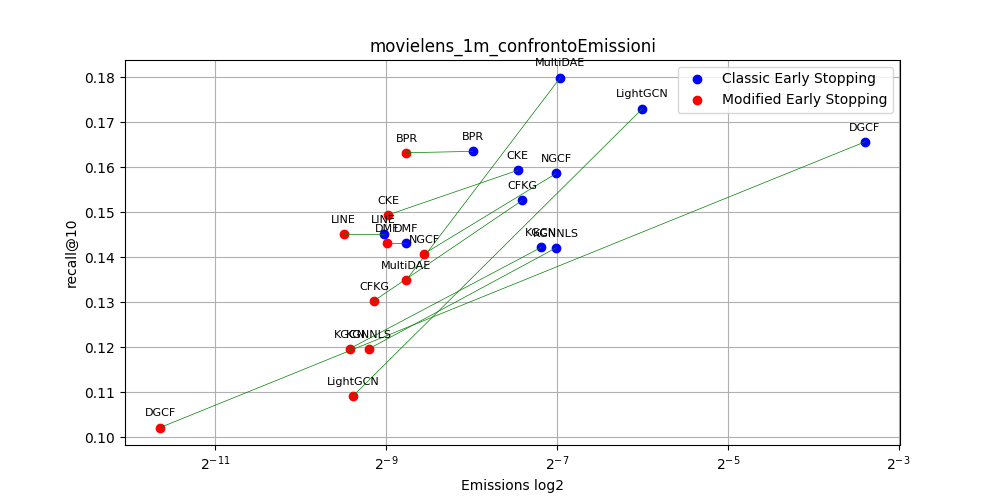
\includegraphics[width=\linewidth, trim=0 0 0 0]{images/recall@10_movielens_1m_comparison.png} &
        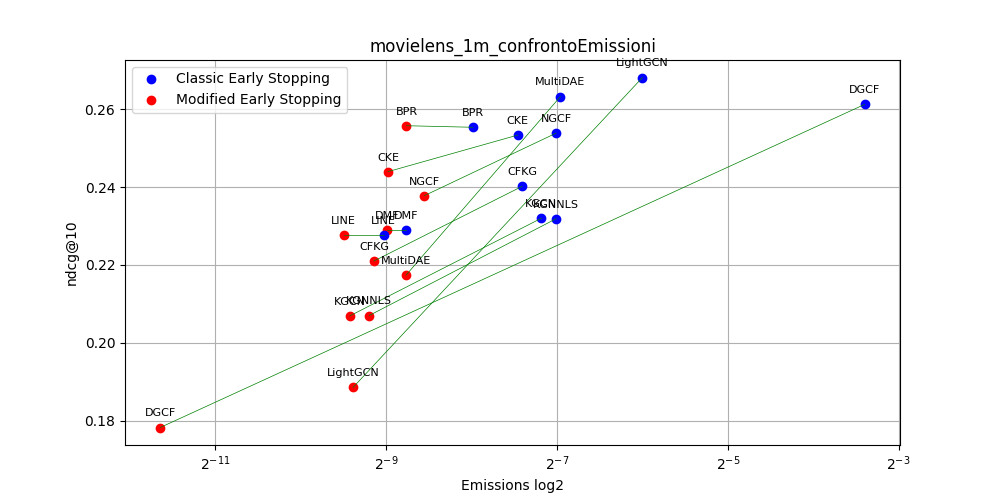
\includegraphics[width=\linewidth, trim=0 0 0 0]{images/ndcg@10_movielens_1m_comparison.png} \\
        \hline
        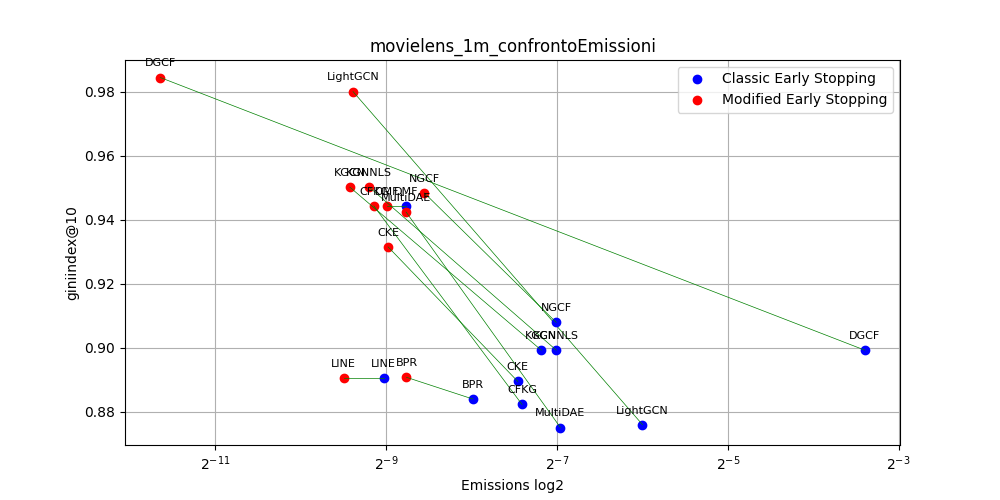
\includegraphics[width=\linewidth, trim=0 0 0 0]{images/giniindex@10_movielens_1m_comparison.png} &
        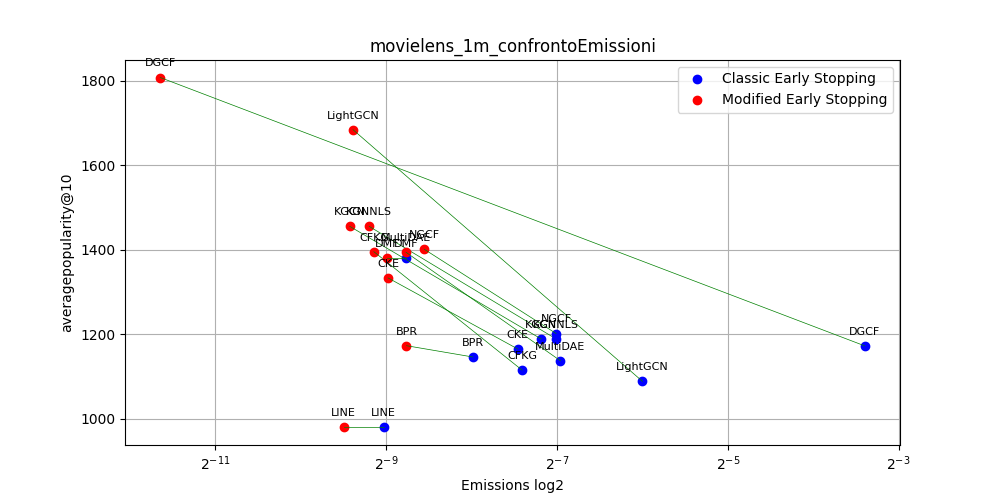
\includegraphics[width=\linewidth, trim=0 0 0 0]{images/averagepopularity@10_movielens_1m_comparison.png} \\
        \hline
    \end{tabularx}
    \caption{Confronto di performance tra criteri}
    \label{tab:emissions_info}
\end{table}




\begin{table}[H]
    \centering
    \resizebox{\textwidth}{!}{
        \begin{tabular}{|c|c|c|c|c|}
            \hline
            \textbf{Modello} & \textbf{Metrica} & \textbf{Score criterio classico} & \textbf{Score criterio nuovo} & \textbf{\% riduzione score}\\
            \hline
            BPR & recall@10 & 0.1635 & 0.1632 & 0.1835\\
            \hline
            CFKG & recall@10 & 0.1526 & 0.1303 & 14.6134\\
            \hline
            CKE & recall@10 & 0.1593 & 0.1494 & 6.2147\\
            \hline
            DMF & recall@10 & 0.1432 & 0.1432 & 0.0\\
            \hline
            KGCN & recall@10 & 0.1422 & 0.1197 & 15.8228\\
            \hline
            KGNNLS & recall@10 & 0.1421 & 0.1197 & 15.7635\\
            \hline
            LINE & recall@10 & 0.1451 & 0.1451 & 0.0\\
            \hline
            MultiDAE & recall@10 & 0.1799 & 0.1349 & 25.0139\\
            \hline
            LightGCN & recall@10 & 0.173 & 0.1092 & 36.8786\\
            \hline
            NGCF & recall@10 & 0.1586 & 0.1408 & 11.2232\\
            \hline
            DGCF & recall@10 & 0.1656 & 0.1022 & 38.2850\\
            \hline
            BPR & ndcg@10 & 0.2554 & 0.2558 & -0.1566\\
            \hline
            CFKG & ndcg@10 & 0.2402 & 0.221 & 7.9933\\
            \hline
            CKE & ndcg@10 & 0.2534 & 0.244 & 3.7096\\
            \hline
            DMF & ndcg@10 & 0.2289 & 0.2289 & 0.0\\
            \hline
            KGCN & ndcg@10 & 0.232 & 0.2069 & 10.819\\
            \hline
            KGNNLS & ndcg@10 & 0.2319 & 0.207 & 10.737\\
            \hline
            LINE & ndcg@10 & 0.2277 & 0.2277 & 0.0\\
            \hline
            MultiDAE & ndcg@10 & 0.2633 & 0.2174 & 17.433\\
            \hline
            LightGCN & ndcg@10 & 0.2682 & 0.1885 & 29.717\\
            \hline
            NGCF & ndcg@10 & 0.2539 & 0.2378 & 6.3411\\
            \hline
            DGCF & ndcg@10 & 0.2613 & 0.1782 & 31.8025\\
            \hline
            BPR & averagepopularity@10 & 1146.3572 & 1173.1199 & -2.3346\\
            \hline
            CFKG & averagepopularity@10 & 1115.4498 & 1395.6098 & -25.1163\\
            \hline
            CKE & averagepopularity@10 & 1165.2413 & 1333.5153 & -14.4411\\
            \hline
            DMF & averagepopularity@10 & 1379.7292 & 1379.7292 & 0.0\\
            \hline
            KGCN & averagepopularity@10 & 1188.9582 & 1455.5651 & -22.4236\\
            \hline
            KGNNLS & averagepopularity@10 & 1188.8981 & 1455.58 & -22.4310\\
            \hline
            LINE & averagepopularity@10 & 979.498 & 979.498 & 0.0\\
            \hline
            MultiDAE & averagepopularity@10 & 1137.4597 & 1394.0944 & -22.5621\\
            \hline
            LightGCN & averagepopularity@10 & 1088.741 & 1684.4149 & -54.7122\\
            \hline
            NGCF & averagepopularity@10 & 1201.8831 & 1401.4325 & -16.6031\\
            \hline
            DGCF & averagepopularity@10 & 1172.6874 & 1807.9828 & -54.1743\\
            \hline
            BPR & giniindex@10 & 0.8839 & 0.8907 & -0.7693\\
            \hline
            CFKG & giniindex@10 & 0.8822 & 0.9443 & -7.0392\\
            \hline
            CKE & giniindex@10 & 0.8894 & 0.9315 & -4.7335\\
            \hline
            DMF & giniindex@10 & 0.9443 & 0.9443 & 0.0\\
            \hline
            KGCN & giniindex@10 & 0.8992 & 0.9502 & -5.6717\\
            \hline
            KGNNLS & giniindex@10 & 0.8992 & 0.9502 & -5.6717\\
            \hline
            LINE & giniindex@10 & 0.8904 & 0.8904 & 0.0\\
            \hline
            MultiDAE & giniindex@10 & 0.875 & 0.9424 & -7.7029\\
            \hline
            LightGCN & giniindex@10 & 0.8759 & 0.9801 & -11.8963\\
            \hline
            NGCF & giniindex@10 & 0.9079 & 0.9484 & -4.4608\\
            \hline
            DGCF & giniindex@10 & 0.8992 & 0.9845 & -9.4862\\
            \hline
        \end{tabular}
    }
    \caption{Confronto degli score tra criteri e modelli}
\end{table}

\noindent Per quanto riguarda giniindex e averagepopularity un punteggio più basso è migliore, mentre per recall e ndcg un punteggio più alto è migliore.
Ecco perchè la percentuale di riduzione degli score è negativa per giniindex e averagepopularity.

\noindent Confrontando le percentuali di riduzione delle emissioni e degli score si può notare la riduzione delle emissioni è molto più alta rispetto alla riduzione degli score.

\noindent BPR tende a mantenere le stesse perfomance con entrambi i criteri a fronte di emissioni molto più basse.
Possiamo notare come LINE e DMF non abbiano subito variazioni di score, mentre LightGCN e DGCF abbiano subito una riduzione molto alta (in percentuale comunque molto inferiore rispetto alla riduzione delle emissioni).
Probabilmente per LINE e DMF il criterio di early stopping classico ha portato ad eseguire qualche epoca in più ma che non ha portato a miglioramenti.

